\section{Introduction}
\label{sec:introduction}

Edge AI aims to improve latency, privacy and decentralize machine learning inference by running models directly on user devices. TinyML \cite{wardenTinyMLMachineLearning2019} focuses on the extreme end of this spectrum, designing models that run on microcontrollers (MCUs). MCUs are severely resource-constrained: typical devices provide one or two CPU cores (usually clocked below 240~MHz) and often 256~KB or less of RAM, preventing them from hosting large models or full-precision weights. Furthermore, low latency is essential because many TinyML applications, such as audio or video streams, require real-time processing.

The extreme memory limitations of microcontrollers make architectural designs with super-linear memory scaling poorly suited for TinyML applications. Consequently, convolutional neural networks (CNNs) and recurrent neural networks (RNNs) have traditionally remained the dominant choices due to their superior parameter efficiency relative to standard multilayer perceptrons (MLPs) or Transformer-based models \cite{trileEfficientNeuralNetworks2026}. However, the recently proposed Mamba architecture \cite{guMambaLinearTimeSequence2024} has emerged as a promising alternative to Transformers for long-context tasks, blending convolutional and recurrent design ideas to capture long-range dependencies while maintaining a linear memory footprint. A high-level diagram of this Mamba block architecture is presented in \autoref{fig:mamba}.

\begin{figure}[ht]
  \centering
  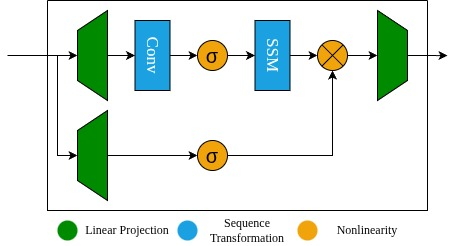
\includegraphics[width=\linewidth]{assets/mamba.jpg}
  \caption{Diagram of the Mamba block.}
  \label{fig:mamba}
\end{figure}

Mamba's main building block is a Selective State-Space Model (S6) layer, which captures long-range structure while avoiding the quadratic complexity of attention.

In Mamba, the S6 matrices are conditioned on the input, allowing the hidden state dynamics to adapt dynamically over time. S6 layers are typically implemented using efficient scan (parallel-prefix) algorithms that parallelize well on modern hardware. However, their recurrent-style execution can make them highly sensitive to quantization and numerical instability
\cite{xuMambaQuantQuantizingMamba2025,tegonFEMBAEdgePhysiologicallyAware2026a}.

Prior work has explored common optimizations for Mamba such as quantization \cite{xuMambaQuantQuantizingMamba2025}, pruning, and knowledge distillation \cite{shihabEfficientUnstructuredPruning}. Notably, MambaLite-Micro \cite{xuMambaLiteMicroMemoryOptimizedMamba2025} implemented PyTorch-style inference for Mamba directly in C and evaluated execution on ESP32-S3 and STM32 microcontrollers. While this verified basic execution feasibility, the implementation is highly model dependent, making deep architectural changes and hardware-specific optimizations cumbersome to explore.

This paper addresses the following overarching research question:
\textit{\textbf{How can Mamba architectures be adapted and optimized for efficient inference on resource-constrained microcontrollers?}}

To address this comprehensively, we formulate three specific sub-questions:
\begin{itemize}
  \item \textbf{RQ1:} What are the primary memory and computational bottlenecks when deploying Mamba models on microcontrollers?
  \item \textbf{RQ2:} How do standard quantization strategies affect Mamba's inference latency, memory footprint, and task accuracy on these edge devices?
  \item \textbf{RQ3:} To what extent can hardware-unfriendly components of the Mamba architecture (e.g., specific activation functions) be simplified or replaced to fit microcontroller constraints, and what are the resulting trade-offs in performance?
\end{itemize}
To answer these questions, we profile deployment strategies on actual hardware, isolate the underlying hardware bottlenecks, and evaluate the efficacy of translating typically GPU-centric optimizations to microcontroller architectures.

The remainder of this paper is organized as follows. Section~\ref{sec:background} surveys related work and foundational background. Section~\ref{sec:methodology} details our proposed optimizations and architectural modifications, while Section~\ref{sec:experimental_setup} outlines how the experiments were conducted. Experimental results are presented in Section~\ref{sec:results}. Their discussion and limitations are described in Section~\ref{sec:discussion}. Finally, Section~\ref{sec:responsible_research} addresses ethical considerations, and Section~\ref{sec:conclusion} concludes the paper with directions for future work.